\chapter{Profiles used and results}
Most of this chapter is taken from \citep{Chaudhary:2020yyv}.

For all these profiles we the spatial domain was [0,2] and the time domain was [0,1].
We used four different profiles of $\psi$,


Gaussian profile:
\[
    \psi(t=0, x)=A \exp \left(\frac{-\left(x-x_{0}\right)^{2}}{\delta^{2}}\right)
\]

Maxwell (or Modified Gaussian) profile:
\[
    \psi(t=0, x)=A x^{2} \exp \left(\frac{-\left(x-x_{0}\right)^{2}}{\delta^{2}}\right)
\]

Ball (or tanh) profile:
\[
    \psi(t=0, x)=A\left(\tanh \left(\frac{-\left(x-x_{0}\right)}{\delta^{2}}\right)+1\right)
\]

Shell profile:
\[
    \psi(t=0, x)=A\left(\tanh \left(\frac{-\left(x-x_{0}\right)}{\delta^{2}}\right)+\tanh \left(\frac{\left(x-x_{0}+w\right)}{\delta^{2}}\right)\right)
\]

For all these profiles we first obtained a rough estimate of the critical amplitude, which was then used to evolve the system once with a subcritical amplitude and then again with a supercritical amplitude.

The simulation was evolved in the supercritical case when it was obvious that the scalar field has moved by $O(1)$ in plank units.

For each profile we are showing two figures, figure (a) shows the fields evolution in time. Blue line is the initial value of $\psi$, green is the value of the field when it reached its maxima at the origin and red is the final value of the field before we stopped the simulation (We stopped the simulations when it was apparent that the field has moved by $O(1)$ distance). Figure (b) shows the value of the field at the origin vs time, blue line shows the subcritical evolution and red line shows the supercritical evolution.

To gain confidence in the results we ran the simulations with multiple step sizes to ensure that the results are independent of the algorithm. In addition to that we also checked the two constraint equations to ensure that the system us evolving correctly.

Subcritical evolution does not involve a lot of field movement thus our algorithm gives very accurate results. But, in the supercritical cases during the collapse the fields start to move very rapidly which leads to a lot of error \ref{chap3:floating_point_errors}.
For the gaussian and the modified gaussian case the constraints had values of the order $10^-5$ at the end.
For the square and the shell profiles the value of the constraint were of the order $10^-3$ at the end of the simulation. These comparatively larger values can be attributed ot the fact that during the collapse field moves much faster in case of square and the shell profiles (Figures \ref{fig:at0_modified_gaussian},\ref{fig:at0_modified_gaussian},\ref{fig:at0_tanh},\ref{fig:at0_shell}).
Although, even in supercritical cases when the field was not moving very fast the constraints were much smaller.

We can decrease the step size to get more accurate results but there is limit on how small one can go due to fixed finite RAM size. One way to deal with this is to use adaptive mesh refinement(AMR), where one reduces the step size at the places where the field is moving very fast to get more accurate results. We decided not to use AMR because writing a AMR code is significantly harder and the accuracy that we were able to achieve was enough to demonstrate our point. That being said with more powerful computers and better algorithms it is possible to achieve much better accuracies if required.



\begin{figure}
    \centering
    \begin{subfigure}[b]{0.85\textwidth}
        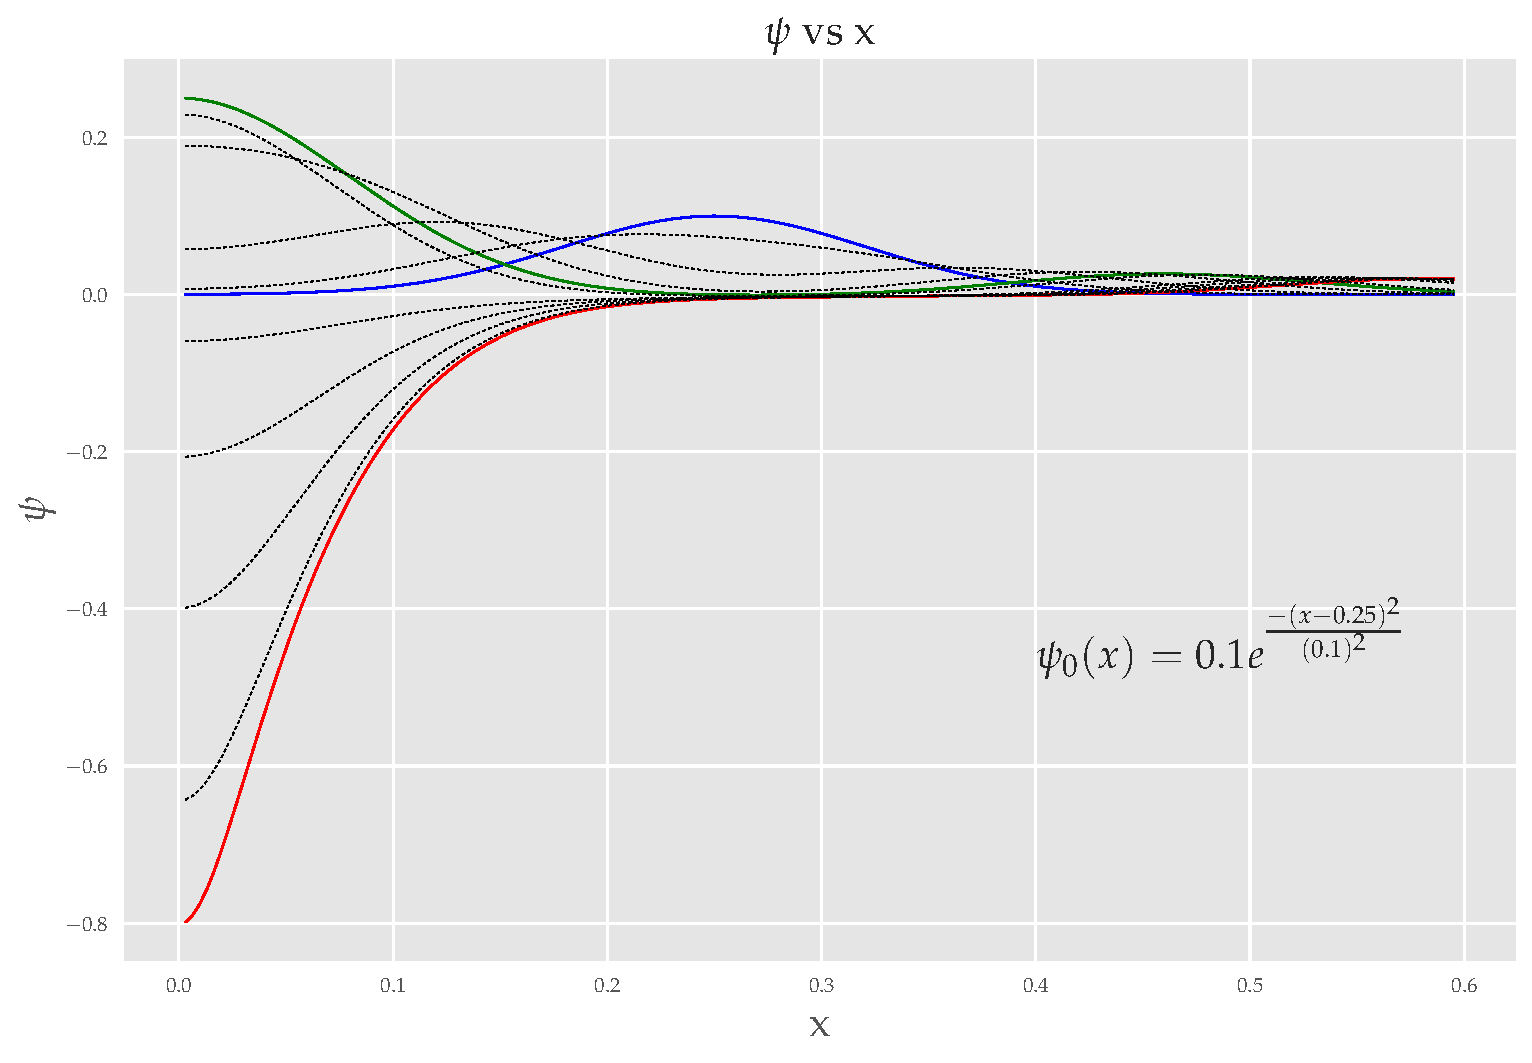
\includegraphics[width=1\linewidth]{images/super_Gaussian.pdf}
        \caption{}
        \label{fig:Ng1}
    \end{subfigure}

    \begin{subfigure}[b]{0.85\textwidth}
        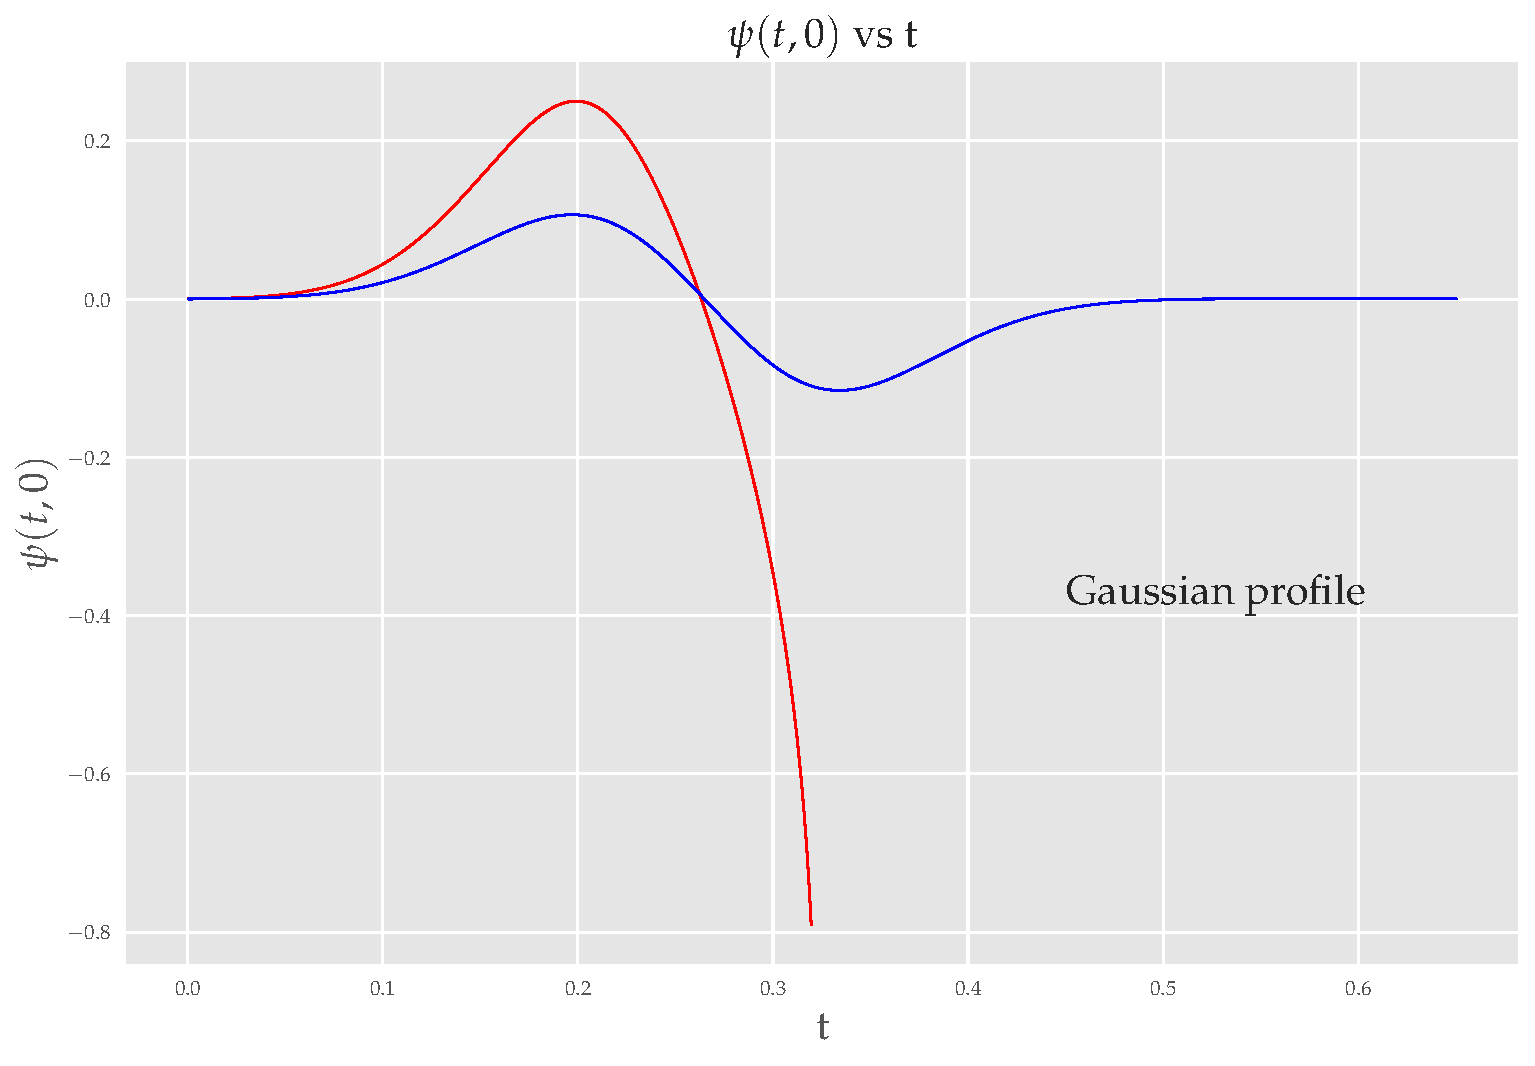
\includegraphics[width=1\linewidth]{images/at0_Gaussian.pdf}w
        \caption{}
        \label{fig:Ng2}
    \end{subfigure}
    \caption[Evolution of $\psi$ from an initial Gaussian profile]{\textbf{Gaussian Profile}. Figure (a) shows supercritical evolution of the field, \textbf{Blue}: initial profile of $\psi$ , \textbf{Green}: profile of $\psi$ when $\psi$ reaches its maxima at the origin, \textbf{Red}: final profile of $\psi$ before the simulation was stopped. Figure (b) shows the supercritical (\textbf{red}) and the subcritical (\textbf{blue}) evolution of $\psi$ at the origin with respect to time.}
\end{figure}



\begin{figure}
    \centering
    \begin{subfigure}[b]{0.85\textwidth}
        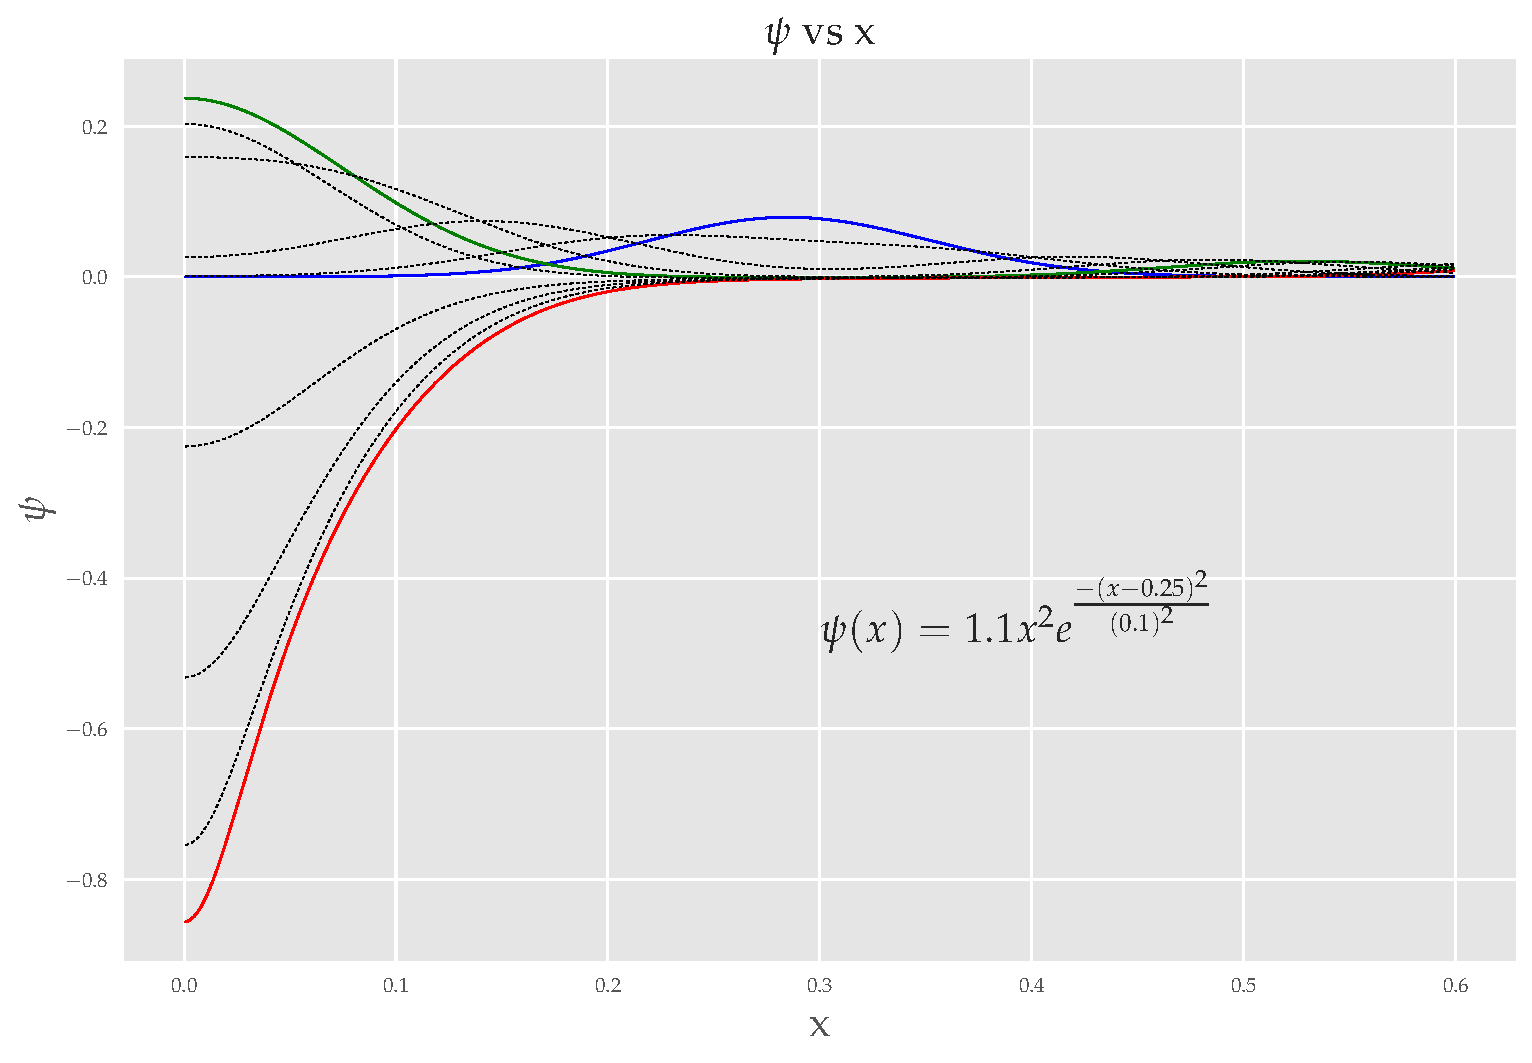
\includegraphics[width=1\linewidth]{images/super_mod.pdf}
        \caption{}
        \label{fig:modified_gaussian}
    \end{subfigure}

    \begin{subfigure}[b]{0.85\textwidth}
        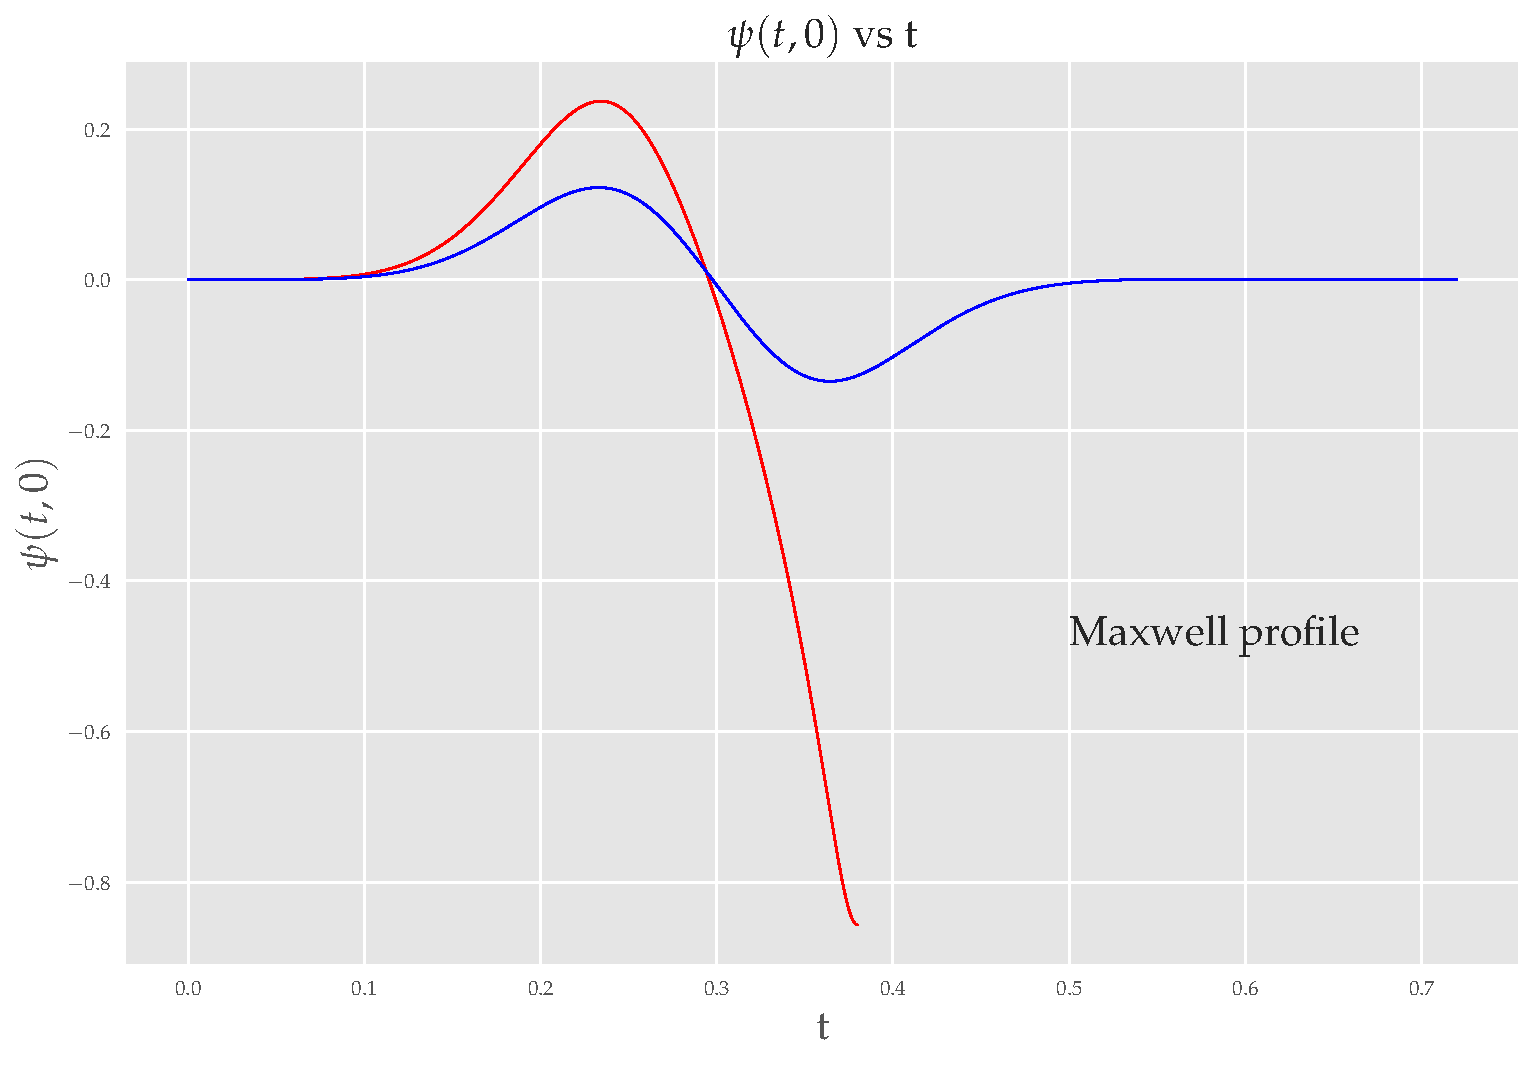
\includegraphics[width=1\linewidth]{images/at0_mod.pdf}
        \caption{}
        \label{fig:at0_modified_gaussian}
    \end{subfigure}
    \caption[Evolution of $\psi$ from an initial Maxwell profile(Modified Gaussian) profile]{\textbf{Maxwell Profile}. Figure (a) shows supercritical evolution of the field, \textbf{Blue}: initial profile of $\psi$ , \textbf{Green}: profile of $\psi$ when $\psi$ reaches its maxima at the origin, \textbf{Red}: final profile of $\psi$ before the simulation was stopped. Figure (b) shows the supercritical (\textbf{red}) and the subcritical (\textbf{blue}) evolution of $\psi$ at the origin with respect to time.}
\end{figure}

\begin{figure}
    \centering
    \begin{subfigure}[b]{0.85\textwidth}
        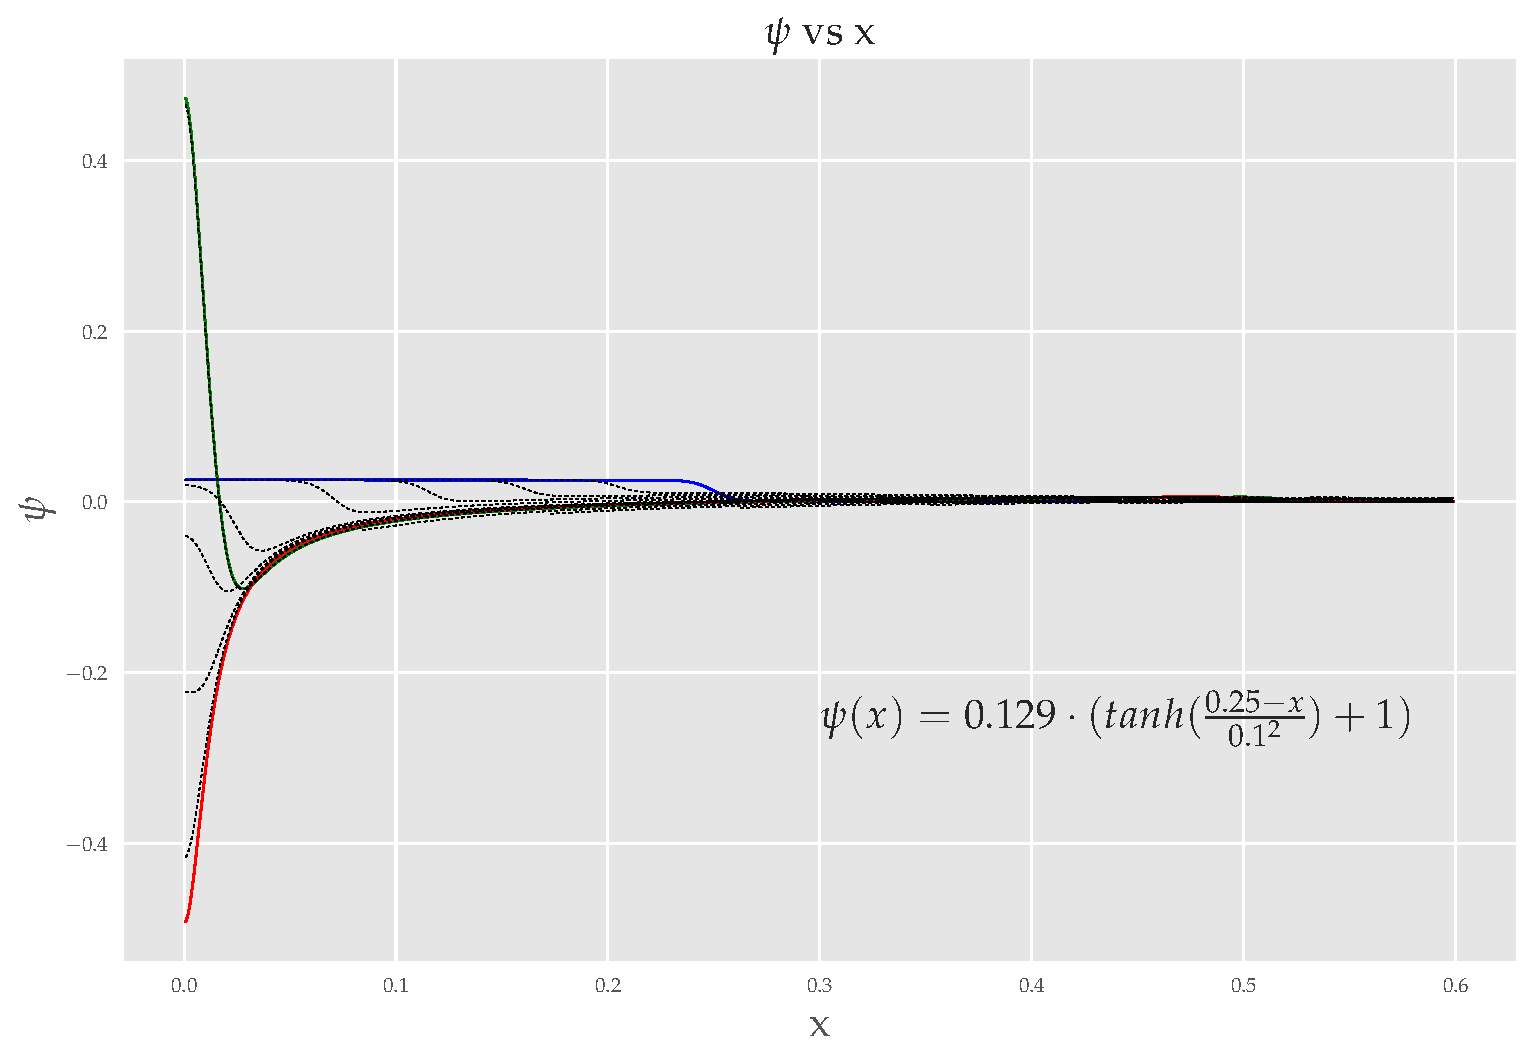
\includegraphics[width=1\linewidth]{images/super_tanh.pdf}
        \caption{}
        \label{fig:tanh}
    \end{subfigure}

    \begin{subfigure}[b]{0.85\textwidth}
        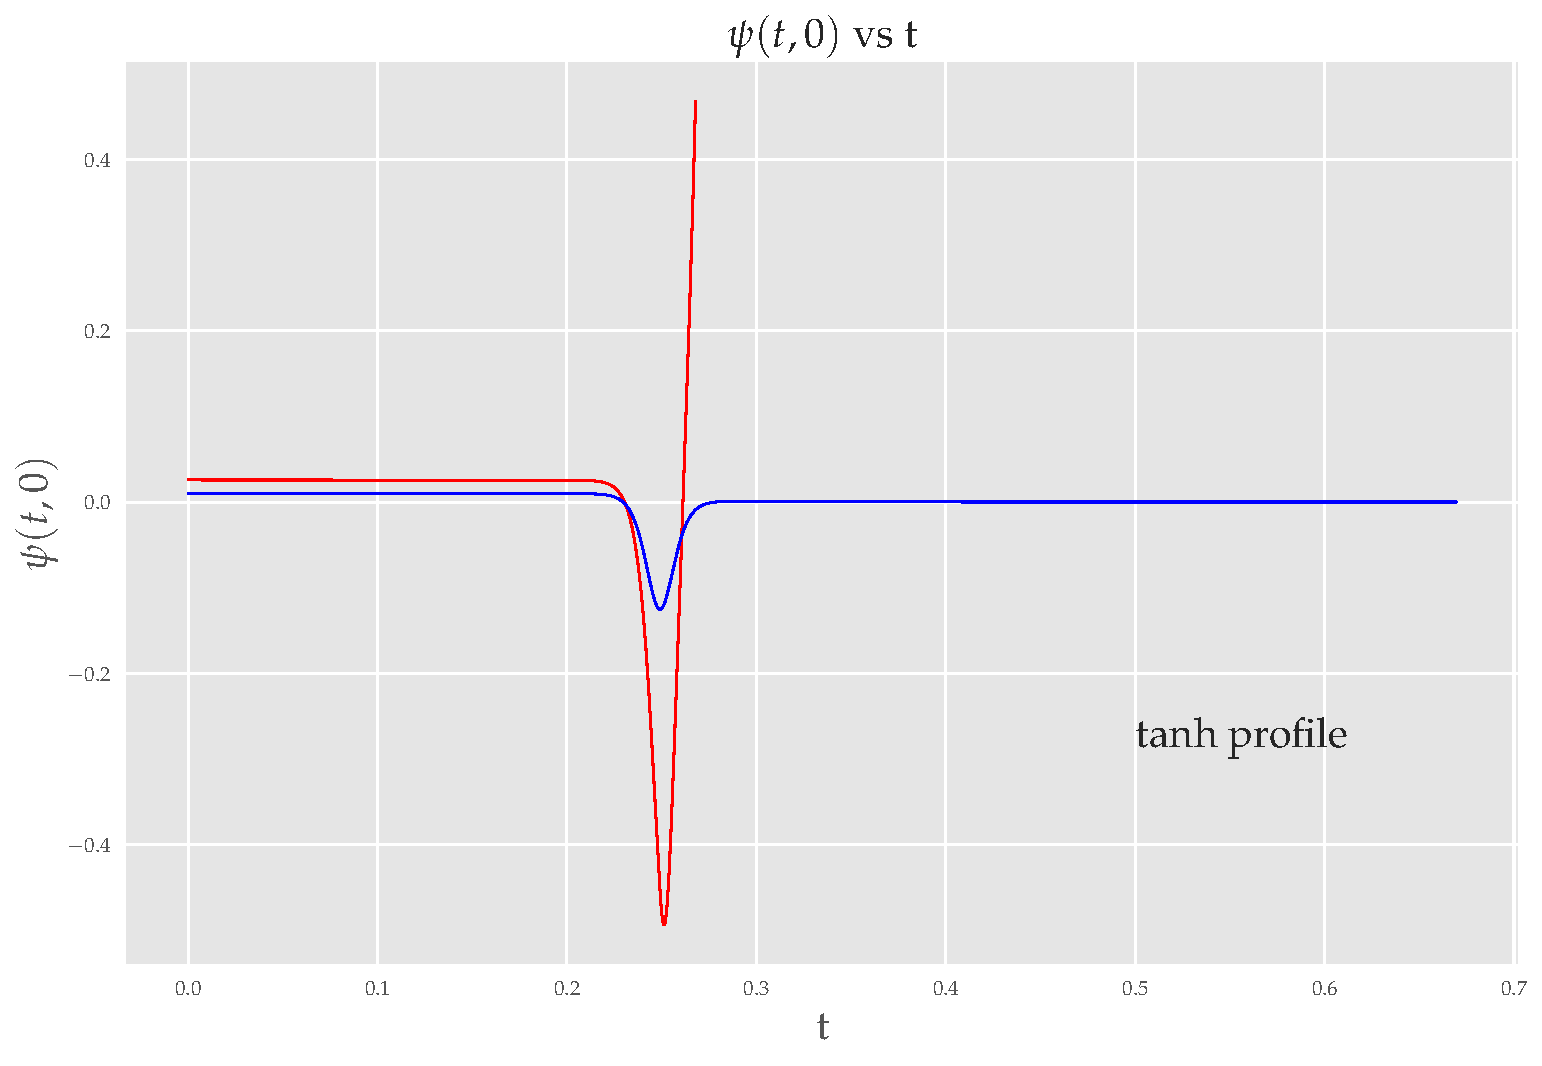
\includegraphics[width=1\linewidth]{images/at0_tanh.pdf}
        \caption{}
        \label{fig:at0_tanh}
    \end{subfigure}
    \caption[Evolution of $\psi$ from an initial tanh profile]{\textbf{Tanh Profile}. Figure (a) shows supercritical evolution of the field, \textbf{Blue}: initial profile of $\psi$ , \textbf{Green}: profile of $\psi$ when $\psi$ reaches its maxima at the origin, \textbf{Red}: final profile of $\psi$ before the simulation was stopped. Figure (b) shows the supercritical (\textbf{red}) and the subcritical (\textbf{blue}) evolution of $\psi$ at the origin with respect to time.}
\end{figure}

\begin{figure}
    \centering
    \begin{subfigure}[b]{0.85\textwidth}
        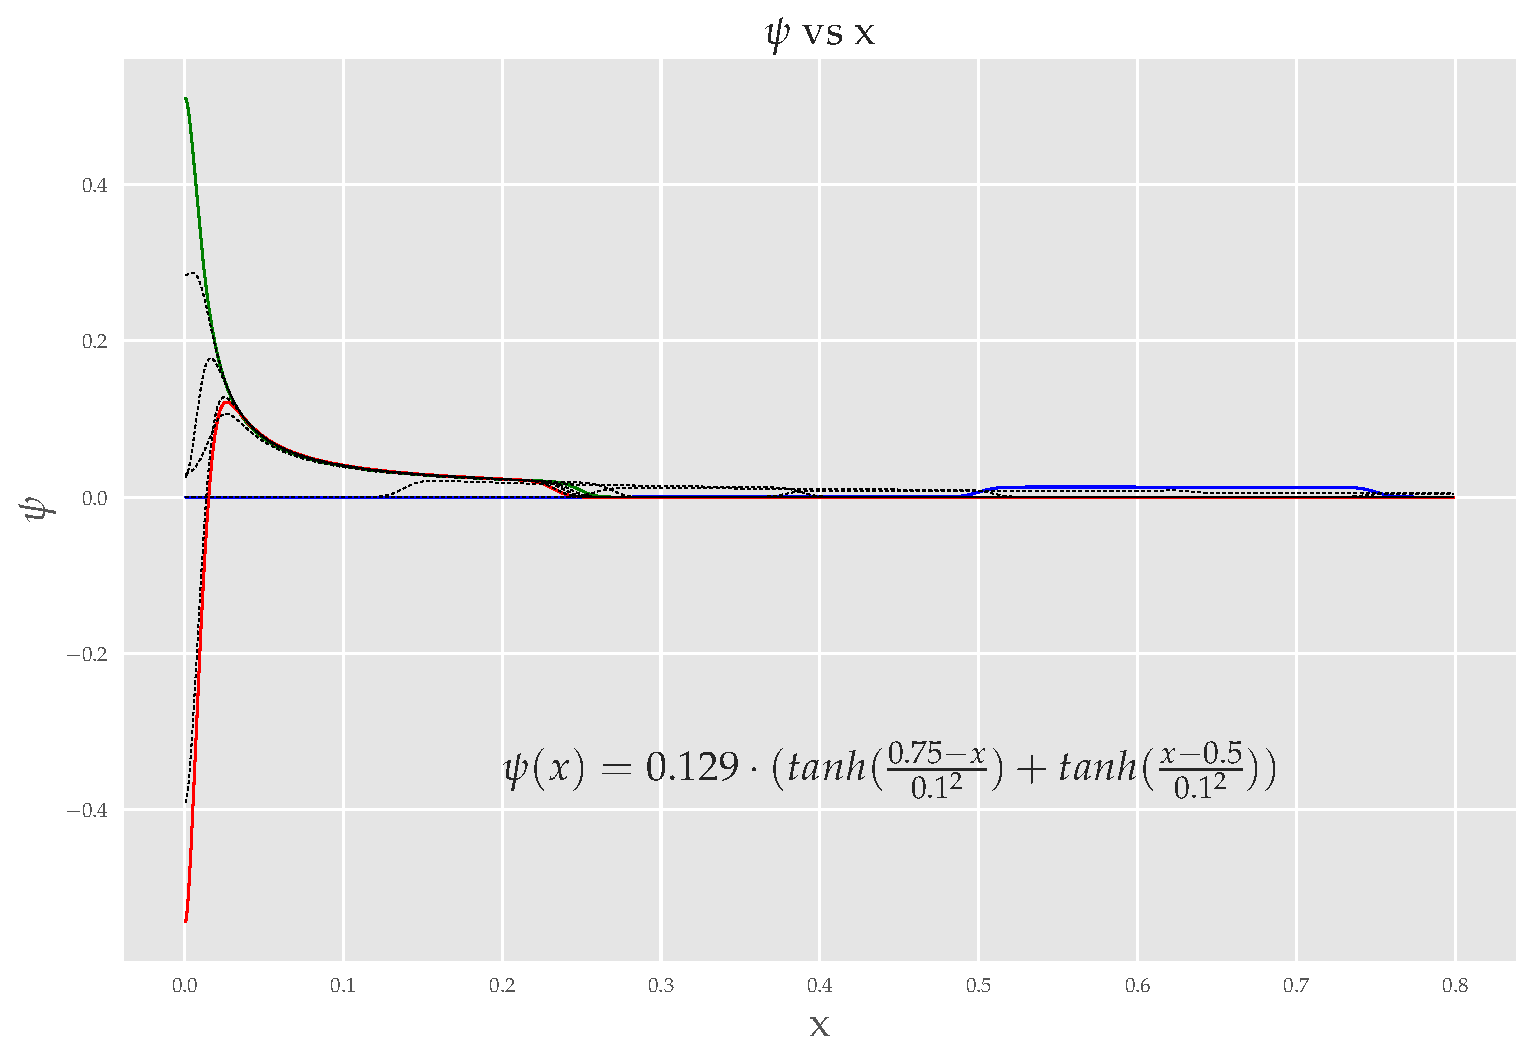
\includegraphics[width=1\linewidth]{images/super_shell.pdf}
        \caption{}
        \label{fig:shell}
    \end{subfigure}

    \begin{subfigure}[b]{0.85\textwidth}
        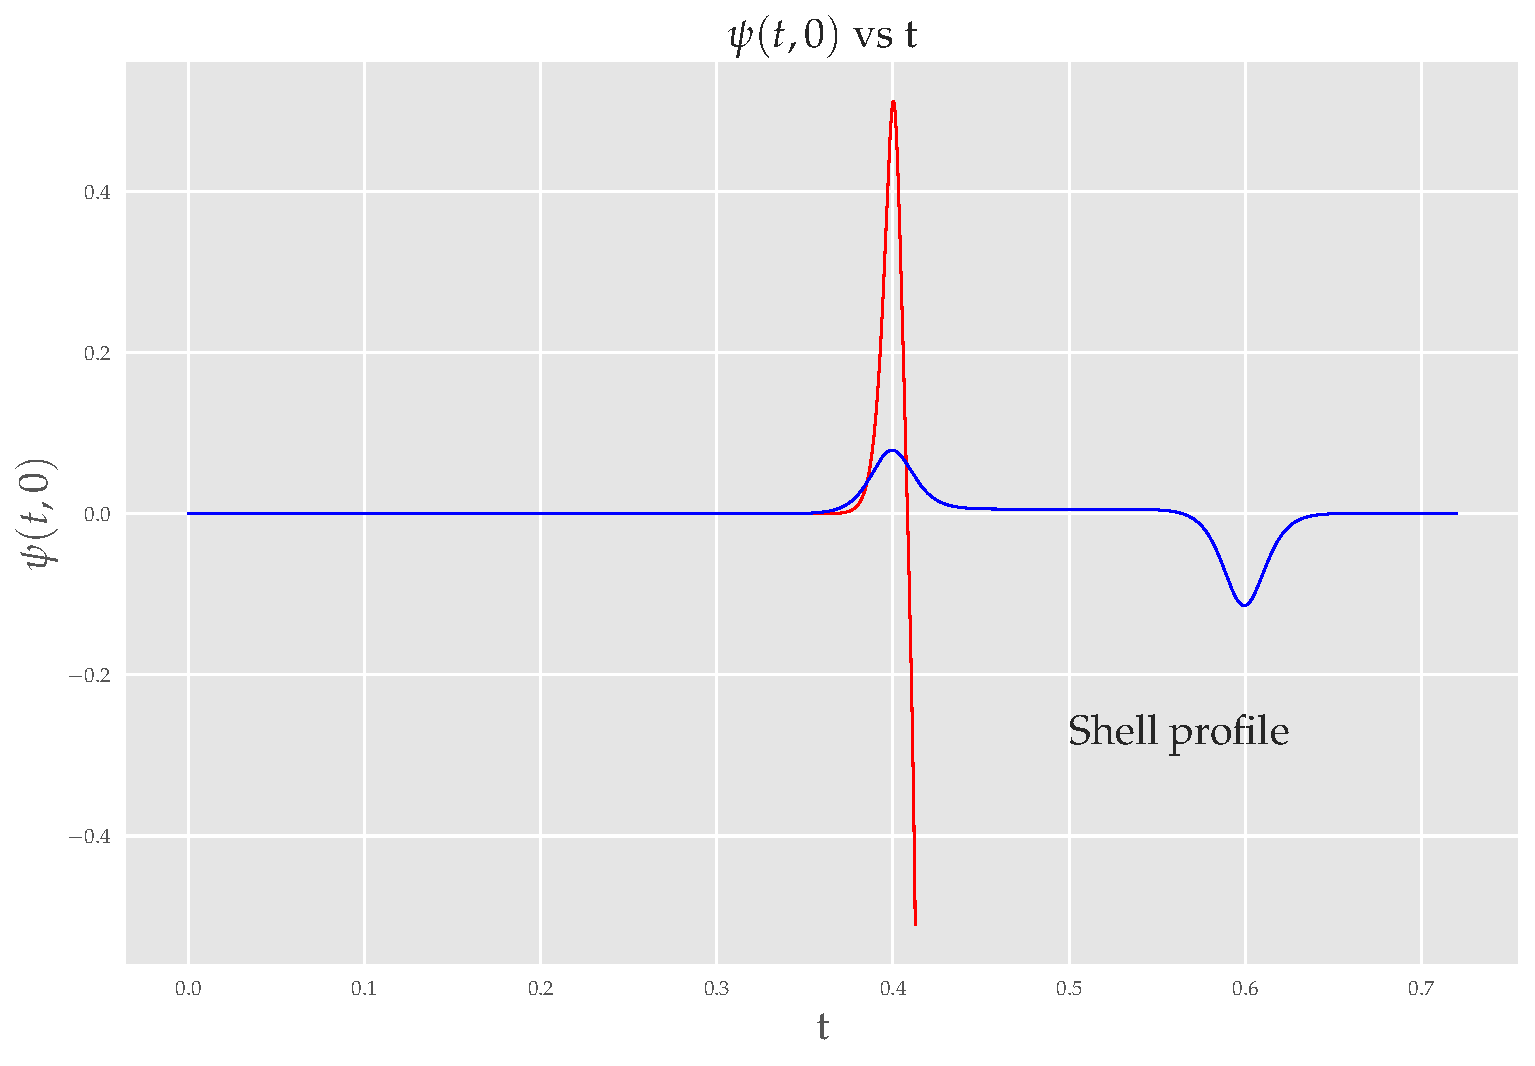
\includegraphics[width=1\linewidth]{images/at0_shell.pdf}
        \caption{}
        \label{fig:at0_shell}
    \end{subfigure}
    \caption[Evolution of $\psi$ from an initial shell profile]{\textbf{Shell Profile}. Figure (a) shows supercritical evolution of the field, \textbf{Blue}: initial profile of $\psi$ , \textbf{Green}: profile of $\psi$ when $\psi$ reaches its maxima at the origin, \textbf{Red}: final profile of $\psi$ before the simulation was stopped. Figure (b) shows the supercritical (\textbf{red}) and the subcritical (\textbf{blue}) evolution of $\psi$ at the origin with respect to time.}
\end{figure}
